\documentclass{standalone}
\usepackage{tikz}
\usepackage{pgfplots}
\pgfplotsset{compat=1.17}

\begin{document}

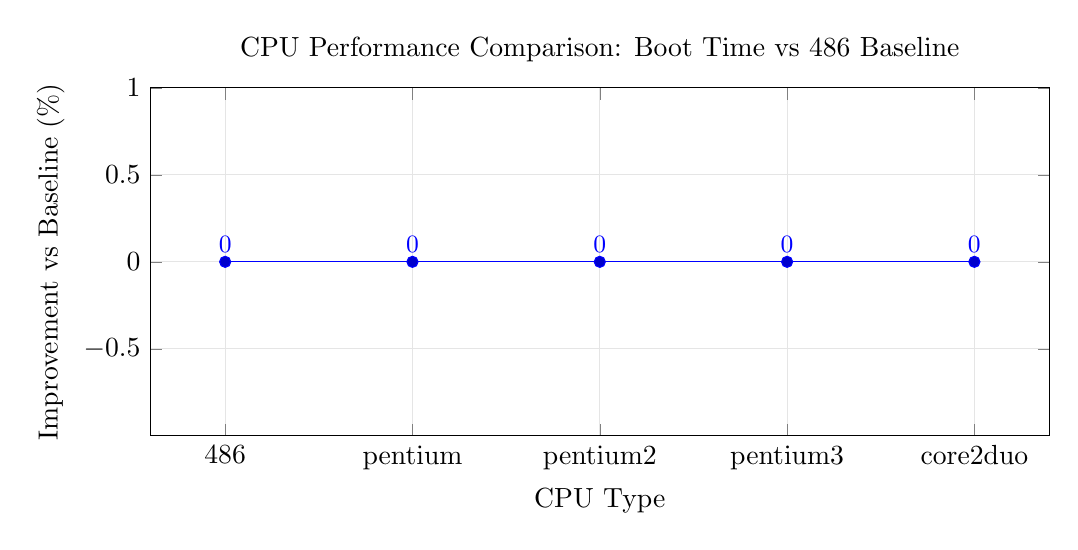
\begin{tikzpicture}
\begin{axis}[
    title={CPU Performance Comparison: Boot Time vs 486 Baseline},
    xlabel={CPU Type},
    ylabel={Improvement vs Baseline (\%)},
    bar width=0.6cm,
    width=13cm,
    height=6cm,
    xtick=data,
    grid=major,
    grid style={gray!20},
    nodes near coords,
    nodes near coords style={font=\small},
    xticklabels={486,pentium,pentium2,pentium3,core2duo}
]

\addplot coordinates {
    (0, 0.0)
    (1, -0.0)
    (2, -0.0)
    (3, -0.0)
    (4, -0.0)

};

\end{axis}
\end{tikzpicture}

\end{document}